% !TEX TS-program = pdflatex
% !TEX encoding = UTF-8 Unicode

% This is a simple template for a LaTeX document using the "article" class.
% See "book", "report", "letter" for other types of document.

\documentclass[11pt]{article} % use larger type; default would be 10pt

\usepackage[utf8]{inputenc} % set input encoding (not needed with XeLaTeX)

%%% Examples of Article customizations
% These packages are optional, depending whether you want the features they provide.
% See the LaTeX Companion or other references for full information.

%%% PAGE DIMENSIONS
\usepackage{geometry} % to change the page dimensions
\geometry{a4paper} % or letterpaper (US) or a5paper or....
% \geometry{margin=2in} % for example, change the margins to 2 inches all round
% \geometry{landscape} % set up the page for landscape
%   read geometry.pdf for detailed page layout information

\usepackage{graphicx} % support the \includegraphics command and options

% \usepackage[parfill]{parskip} % Activate to begin paragraphs with an empty line rather than an indent

%%% PACKAGES
\usepackage{booktabs} % for much better looking tables
\usepackage{array} % for better arrays (eg matrices) in maths7
\usepackage{amsmath}
\usepackage{hyperref}
\usepackage{paralist} % very flexible & customisable lists (eg. enumerate/itemize, etc.)
\usepackage{verbatim} % adds environment for commenting out blocks of text & for better verbatim
\usepackage{subfig} % make it possible to include more than one captioned figure/table in a single float
% These packages are all incorporated in the memoir class to one degree or another...

%%% HEADERS & FOOTERS
\usepackage{fancyhdr} % This should be set AFTER setting up the page geometry
\pagestyle{fancy} % options: empty , plain , fancy
\renewcommand{\headrulewidth}{0pt} % customise the layout...
\lhead{}\chead{}\rhead{}
\lfoot{}\cfoot{\thepage}\rfoot{}

%%% SECTION TITLE APPEARANCE
\usepackage{sectsty}
\allsectionsfont{\sffamily\mdseries\upshape} % (See the fntguide.pdf for font help)
% (This matches ConTeXt defaults)

%%% ToC (table of contents) APPEARANCE
\usepackage[nottoc,notlof,notlot]{tocbibind} % Put the bibliography in the ToC
\usepackage[titles,subfigure]{tocloft} % Alter the style of the Table of Contents
\renewcommand{\cftsecfont}{\rmfamily\mdseries\upshape}
\renewcommand{\cftsecpagefont}{\rmfamily\mdseries\upshape} % No bold!

%%% END Article customizations

%%% The "real" document content comes below...

\title{Report group 0}
\author{Niclas, Samuel, Hanif, Joshua}
%\date{} % Activate to display a given date or no date (if empty),
         % otherwise the current date is printed 

\begin{document}
\maketitle

\begin{abstract}
In this document we present an implementiation of a autonomous robot capable of interacting with an unknown environment and performing certain predefined tasks which involves ''obstacle avoidance'', ''tag detection \& classification'', ''map creation and localization'' and ''path planing/finding''.
\end{abstract}

\newpage
\tableofcontents

\clearpage
\section{Introduction}
....

\section{Hardware and mechanical design}
\subsection{Hardware used}

For the construction of our robot we were given the following components, not all of them were used in the final construction:
\begin{itemize}
\item Roboard (Roboard-100) (used)
\item Serializer board (used)
\item Custom made powerboard (used)
\item 2 motors with encoders (2 used)
\item 2 wheels for each side (2 used)
\item 2 caster wheels (1 used)
\item Aluminum plates (used)
\item Sonar (Devantech SRF08) (used)
\item 2 web cameras (Logitech C905) (1 used)
\item 8+ short range/long range IR-sensors (Sharp GP2D120XJ00F/GP2D12J0000F) (6 short and 2 long range used)
\item Wireless USB Adapter (Belkin P-F5D8053) (used)
\item Battery(LiPo) with charger(team Orion advantage IQ605) (used)
\item Lots of wires and other stuff that was needed to mount everything
\item 2 Servo (not used)
\item IMU (not used)
\item Bumbers (not used)
\end{itemize}


\subsection{Mechanical Design}

Before start designing and building the robot, there were some constraints to consider:
\begin{itemize}
\item The robot can not be wider than 40 cm and it can not be taller than 29 cm.
\item It must be fairly circular to avoid hitting obstacles when rotating.
\item The camera must be placed in such way that it can detect tags that are placed at least 10 cm and at most 25 cm from the floor.
\item The IR-sensors must be fitted inside the error threshold.
\end{itemize}
Besides the constraints above, we decided to not build everything at once but to build the basics in such way that we can easily add and make changes to it. This resultet in several changes for the placement of the sensors.
The basic design was also drawn in a 3D modelling program (Google Sketchup) to test different configuration before actually putting them together.

\begin{figure}[h]
\label{fig:google_sketchup_draw1}
    \begin{centering}
   	 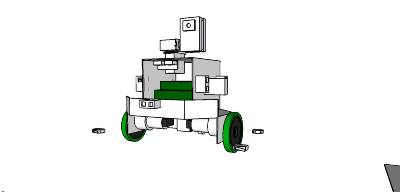
\includegraphics[scale=0.5]{figures/g_sketchup_v7.jpeg}
   	 \caption{The final 3D model version in Google Sketchup}\label{fig:google_sketchup_draw1}
    \end{centering}
\end{figure}


\begin{figure}[h]
\label{fig:amee_final}
    \begin{centering}
   	 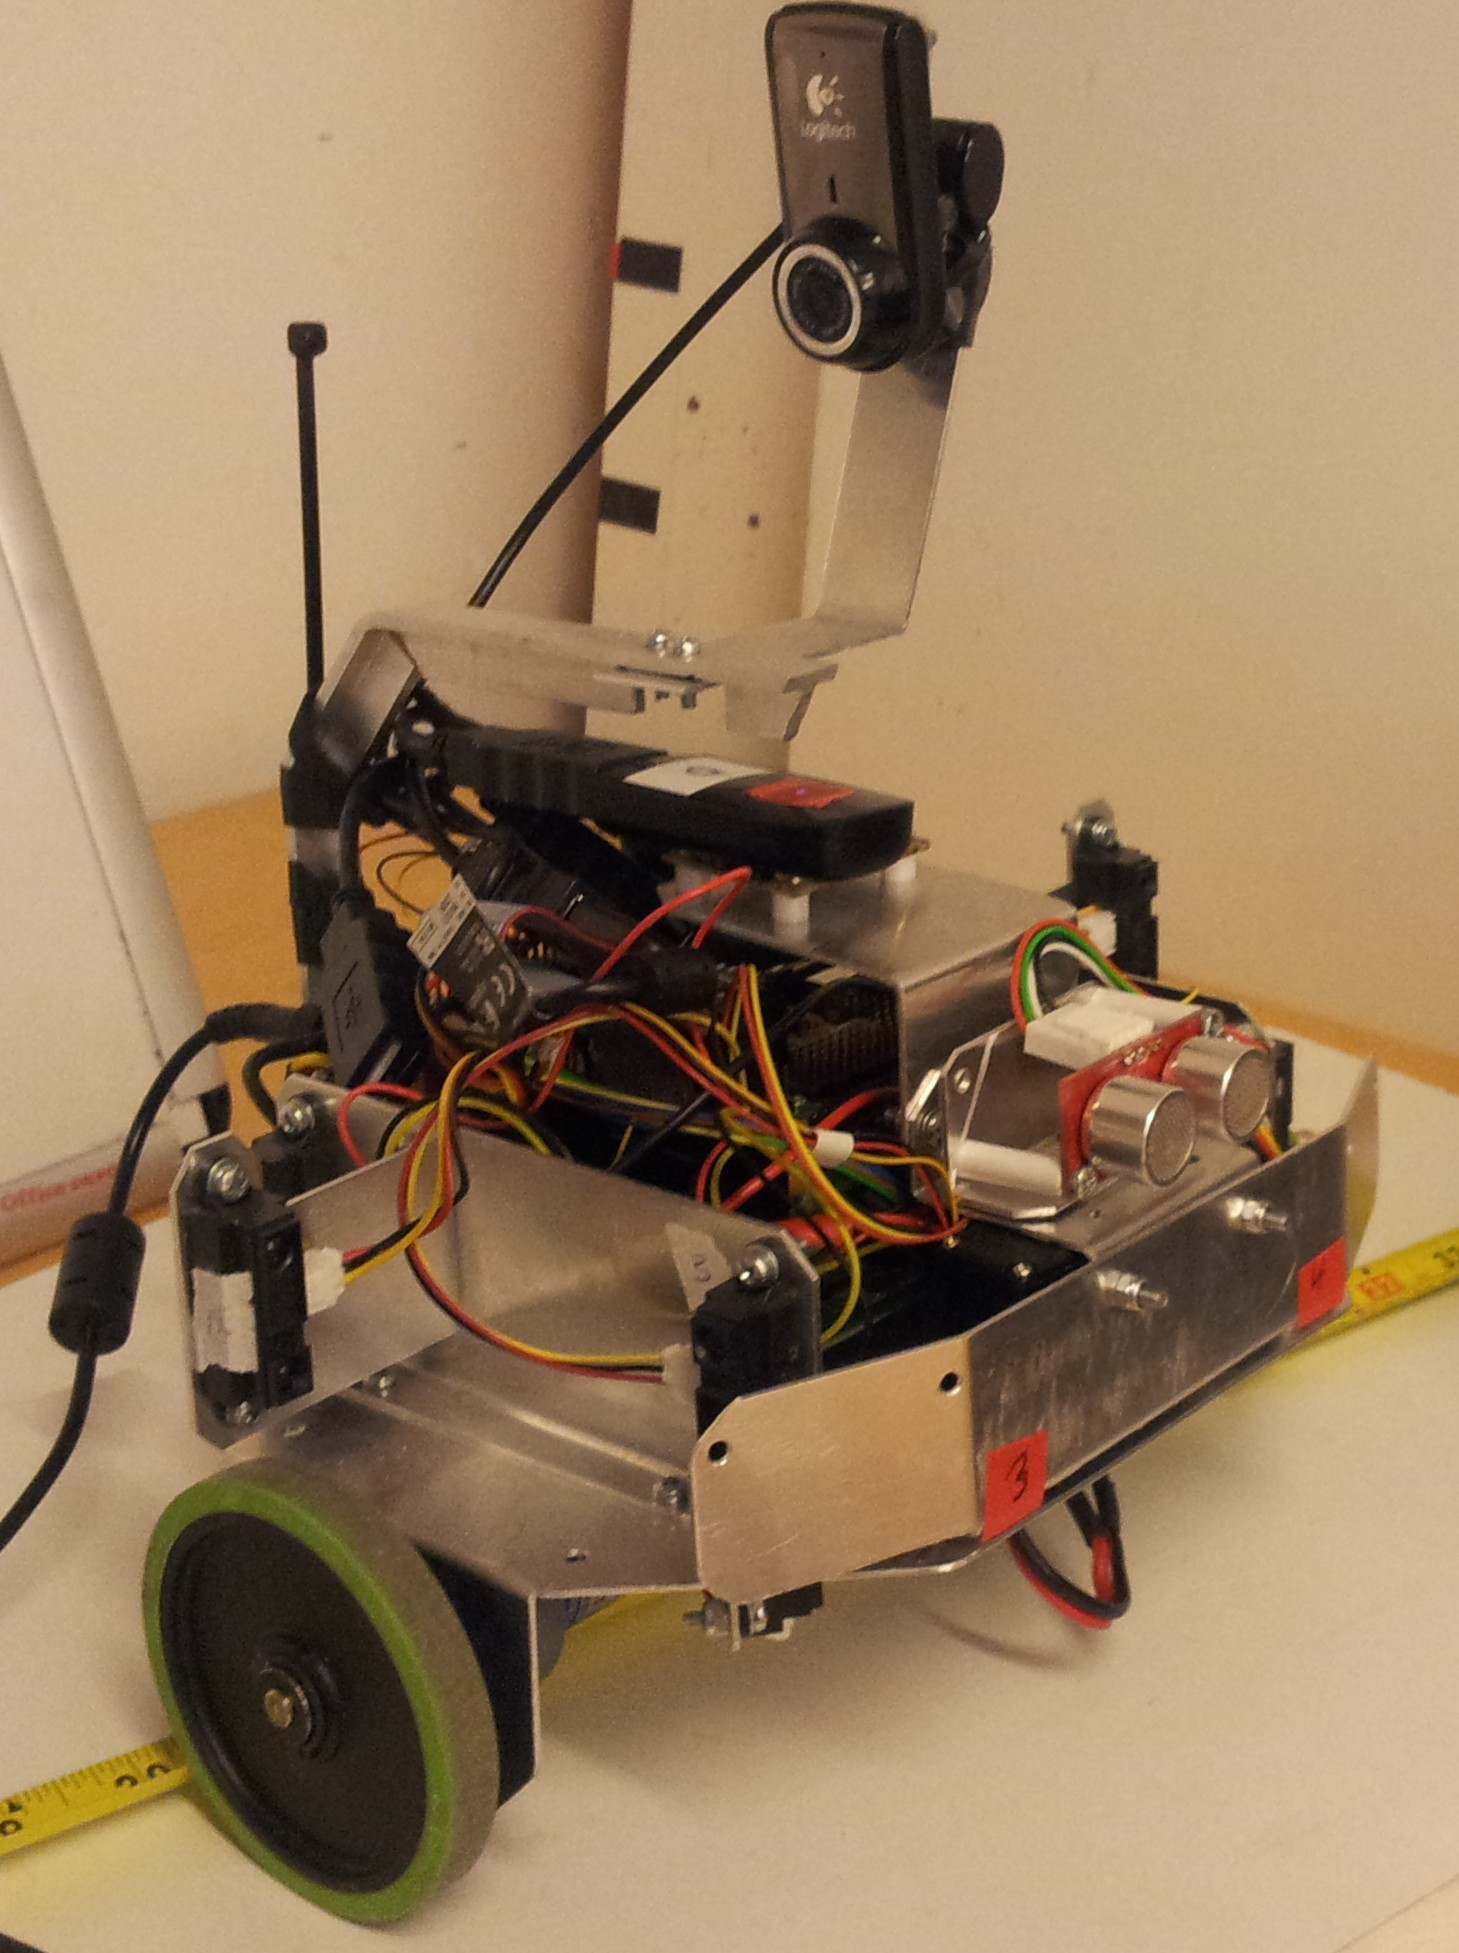
\includegraphics[scale=0.5]{figures/amee_final.jpg}
   	 \caption{The final hardware design}\label{fig:amee_final}
    \end{centering}
\end{figure}

\subsection{Sensors}

Sensors are used to tell the robot what happens in it's surrounding or how it has moved. 
In order to achieve a proper movement control, sensor feedback is required so that the controlling unit can know what the actuators actually do with the control signal. There is a delay in the actuation, since motors doesn't react instantly on a voltage applied to it, and also some uncertainty. This robot make use of 3 different types of sensors to sense the environment and localize itself. The sensors are listed and explained below:
\begin{itemize}
\item Wheel encoders outputs tics where each tic corresponds to a certain rotation of the motor axis. The tics are converted to a distance so that the movement can be determined. The movement is integrated over time so that a position and heading is obtained with respect to the starting position and heading. However, the odometry is not perfect since the wheels slip when the robot turns, accelerates and brakes. 

\item IR sensor outputs a voltage that is based on the reflected intensity of the reflected light. This voltage is then read by the robot's analog to digital converter and the voltage is translated into a distance. This measurement doesn't have any drift since the measurement is relative to a wall and not something that is integrated over time. However the downside is that the reflections can be misleading if it reflects from an edge or a different material. It is also limited in the measuring range.

\item Sonar sensor which measures the distance to the closest obstacle in front of it. This could be used for detecting small obstacles in front of the robot since it sees an area in front of the robot and not just in a line as the IR sensors do.

\item A fourth sensor is a camera and is used for finding and classifying tags. This is further described in section \ref{sect:computerVision}.

\end{itemize}

\section{Software}
This section describes the software that we used, a class diagram of our implementation and a flow chart of how the robot interacts with its environment.

\subsection{Software used}
The robot needs to execute multiple tasks and react on many inputs at once. Therefore we were recomended to use Robot Operating System (ROS) which is a software framework that can be run on other *nix-like operating systems like GNU/Linux and Mac OS X. ROS basically works as a intermediate ``talker'' between the different processes that we run on our robot. The advantage of using ROS instead of explicitally create threads that can comunicate with each other is that we can rather simple separate each functionality and test them seperately. It also unsure that we don't need to handle deadlocks and shared objects. The drawbacks are the time it takes to get a good grep of how ROS works, and that it has a slight overhead compared to pthread library.

Other software that we used were:
\begin{itemize}
\item Git for version controlling.
\item Gcc for compiling our C-code.
\item Python 2.7 for running some scripts and for map visualization.
\item OpenCV for computer vision.
\item Google Sketchup for drawing 3D models.
\item Fabric, a python library, for copying binany files from the workstation to the robot.
\end{itemize}

\subsection{Software Structure}
We started to implement some highlevel part (MovementController) in python, but later found out that it was too slow to run on the hardware that we currently have. By translating the code directly to C++, we could see a huge difference in performance.

Through the whole project, we had to restructure our code multiple times. This was partly because we did not know what problem we could encounter. For example we had to add many movement states for the robot to handle all the type of movements that we had not thought of.

Below you can see a flowchart of the final implementation.

\begin{figure}[h!]
\label{fig:flow_chart}
    \begin{centering}
   	 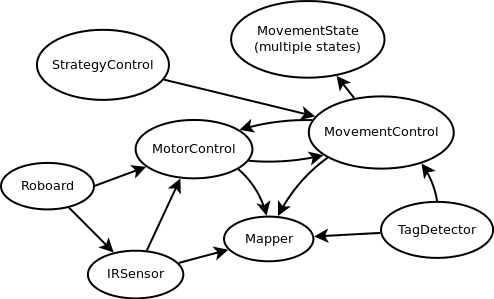
\includegraphics[scale=0.5]{figures/flow_chart.png}
   	 \caption{A flow chart of how the different processes interact}\label{fig:flow_chart}
    \end{centering}
\end{figure}



\section{Motion control}
The motion control is meant to give the robot a smooth and accurate movement that enables wall following and movement through most environments that could appear with the given constraints on the environment.

\subsection{Motor control}

The low level control is performed by the motor control. It receives a velocity message (right speed and left speed) and tries to keep the reference speeds by feeding them into two controllers, one for each wheel. The controllers takes the error (reference speed minus actual speed) and multiplies it with a constant that is tuned manually to obtain a good control performance. This type of controller is called a P-controller (P for proportional). The actual speed is calculated from the time derivative of the wheel encoder measurements and then subtracted from the reference speed to get the error.
With a steady speed the robot can be assumed to either move in a straight line or rotate on the spot depending on the reference signal.

\subsection{Angular and linear movement }

The two basic movements that are needed to explore the whole environment are rotation on the spot and moving straight. Rotation is performed by a P-controller that computes a control signal based on the difference between the reference angle and the actual angle. The angular speed is also saturated to prevent unreasonable high or low speeds. Further, the motion is smoothed by applying an acceleration phase while starting a rotation movement and a lower acceleration results in less wheel slippage and thereby a more accurate final angle. The output (rotation speed) from the rotation function is sent to one motor, and the other gets the rotation speed with switched sign. The architecture of the control system for rotation is shown in figure \ref{fig:rotation_blockdiagram}.

\begin{figure}[h]
\label{fig:rotation_blockdiagram}
    \begin{centering}
   	 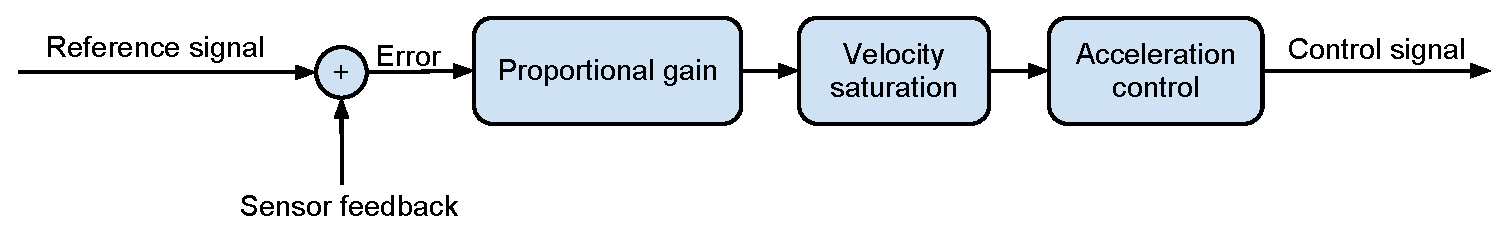
\includegraphics[scale=0.5]{figures/rotate_blockdiagram.pdf}
   	 \caption{Controller architecture for rotate function.}\label{fig:rotation_blockdiagram}
    \end{centering}
\end{figure}

The straight movement is based on the same idea but instead of sending a positive speed on one wheel and a negative on the other, both speeds have the same sign to either move the robot backwards or forward. 

\subsection{Wall following}
\label{subsec:wallFollowing}

Wall following moves the robot along a wall and makes it turn so that most situations can be handled. The wall following node is using the previously mentioned functionalities, linear movement and angular movement, to be able to follow the wall. In addition to the encoder measurements it now uses the IR sensors to determine the distance and an angle to the wall. These measurements have the benefit of having a absolute error compared to the encoder measurements that drifts over time and the error integrates and eventually becomes very large.
	The sensor input is sent to a P-controller that controls the angle to the wall, so that the robot drives parallel to the wall, this makes the robot move in a fairly straight line while doing wall following. The distance to the wall is only controlled in case the robot exceeds a threshold of being too close or too far from the wall. This makes the robot behave smoother and do less corrections to keep the right distance and will also improve the odometry since the robot will turn less.
	The wall following functionality is based on a state machine that changes state when the wall cannot be followed any more without further actions. The state machine is shown in figure  \ref{fig:followWallStates} and the states are designed to handle most tricky situations that can appear in the environment. Conditions used in the state machine are explained in table \ref{table:conditions}.

\begin{table}
\label{table:conditions}
\center
  \begin{tabular}{l|l}
    % \hline
    \textbf{Condition} & \textbf{Description} \\ \hline
    rF & Right front IR sensor sees a wall \\ \hline
    rL & Right left IR sensor sees a wall \\ \hline
    WF & Wall in front detected \\
    \hline
  \end{tabular}
\end{table}

\begin{figure}[h]
    \begin{centering}
   	 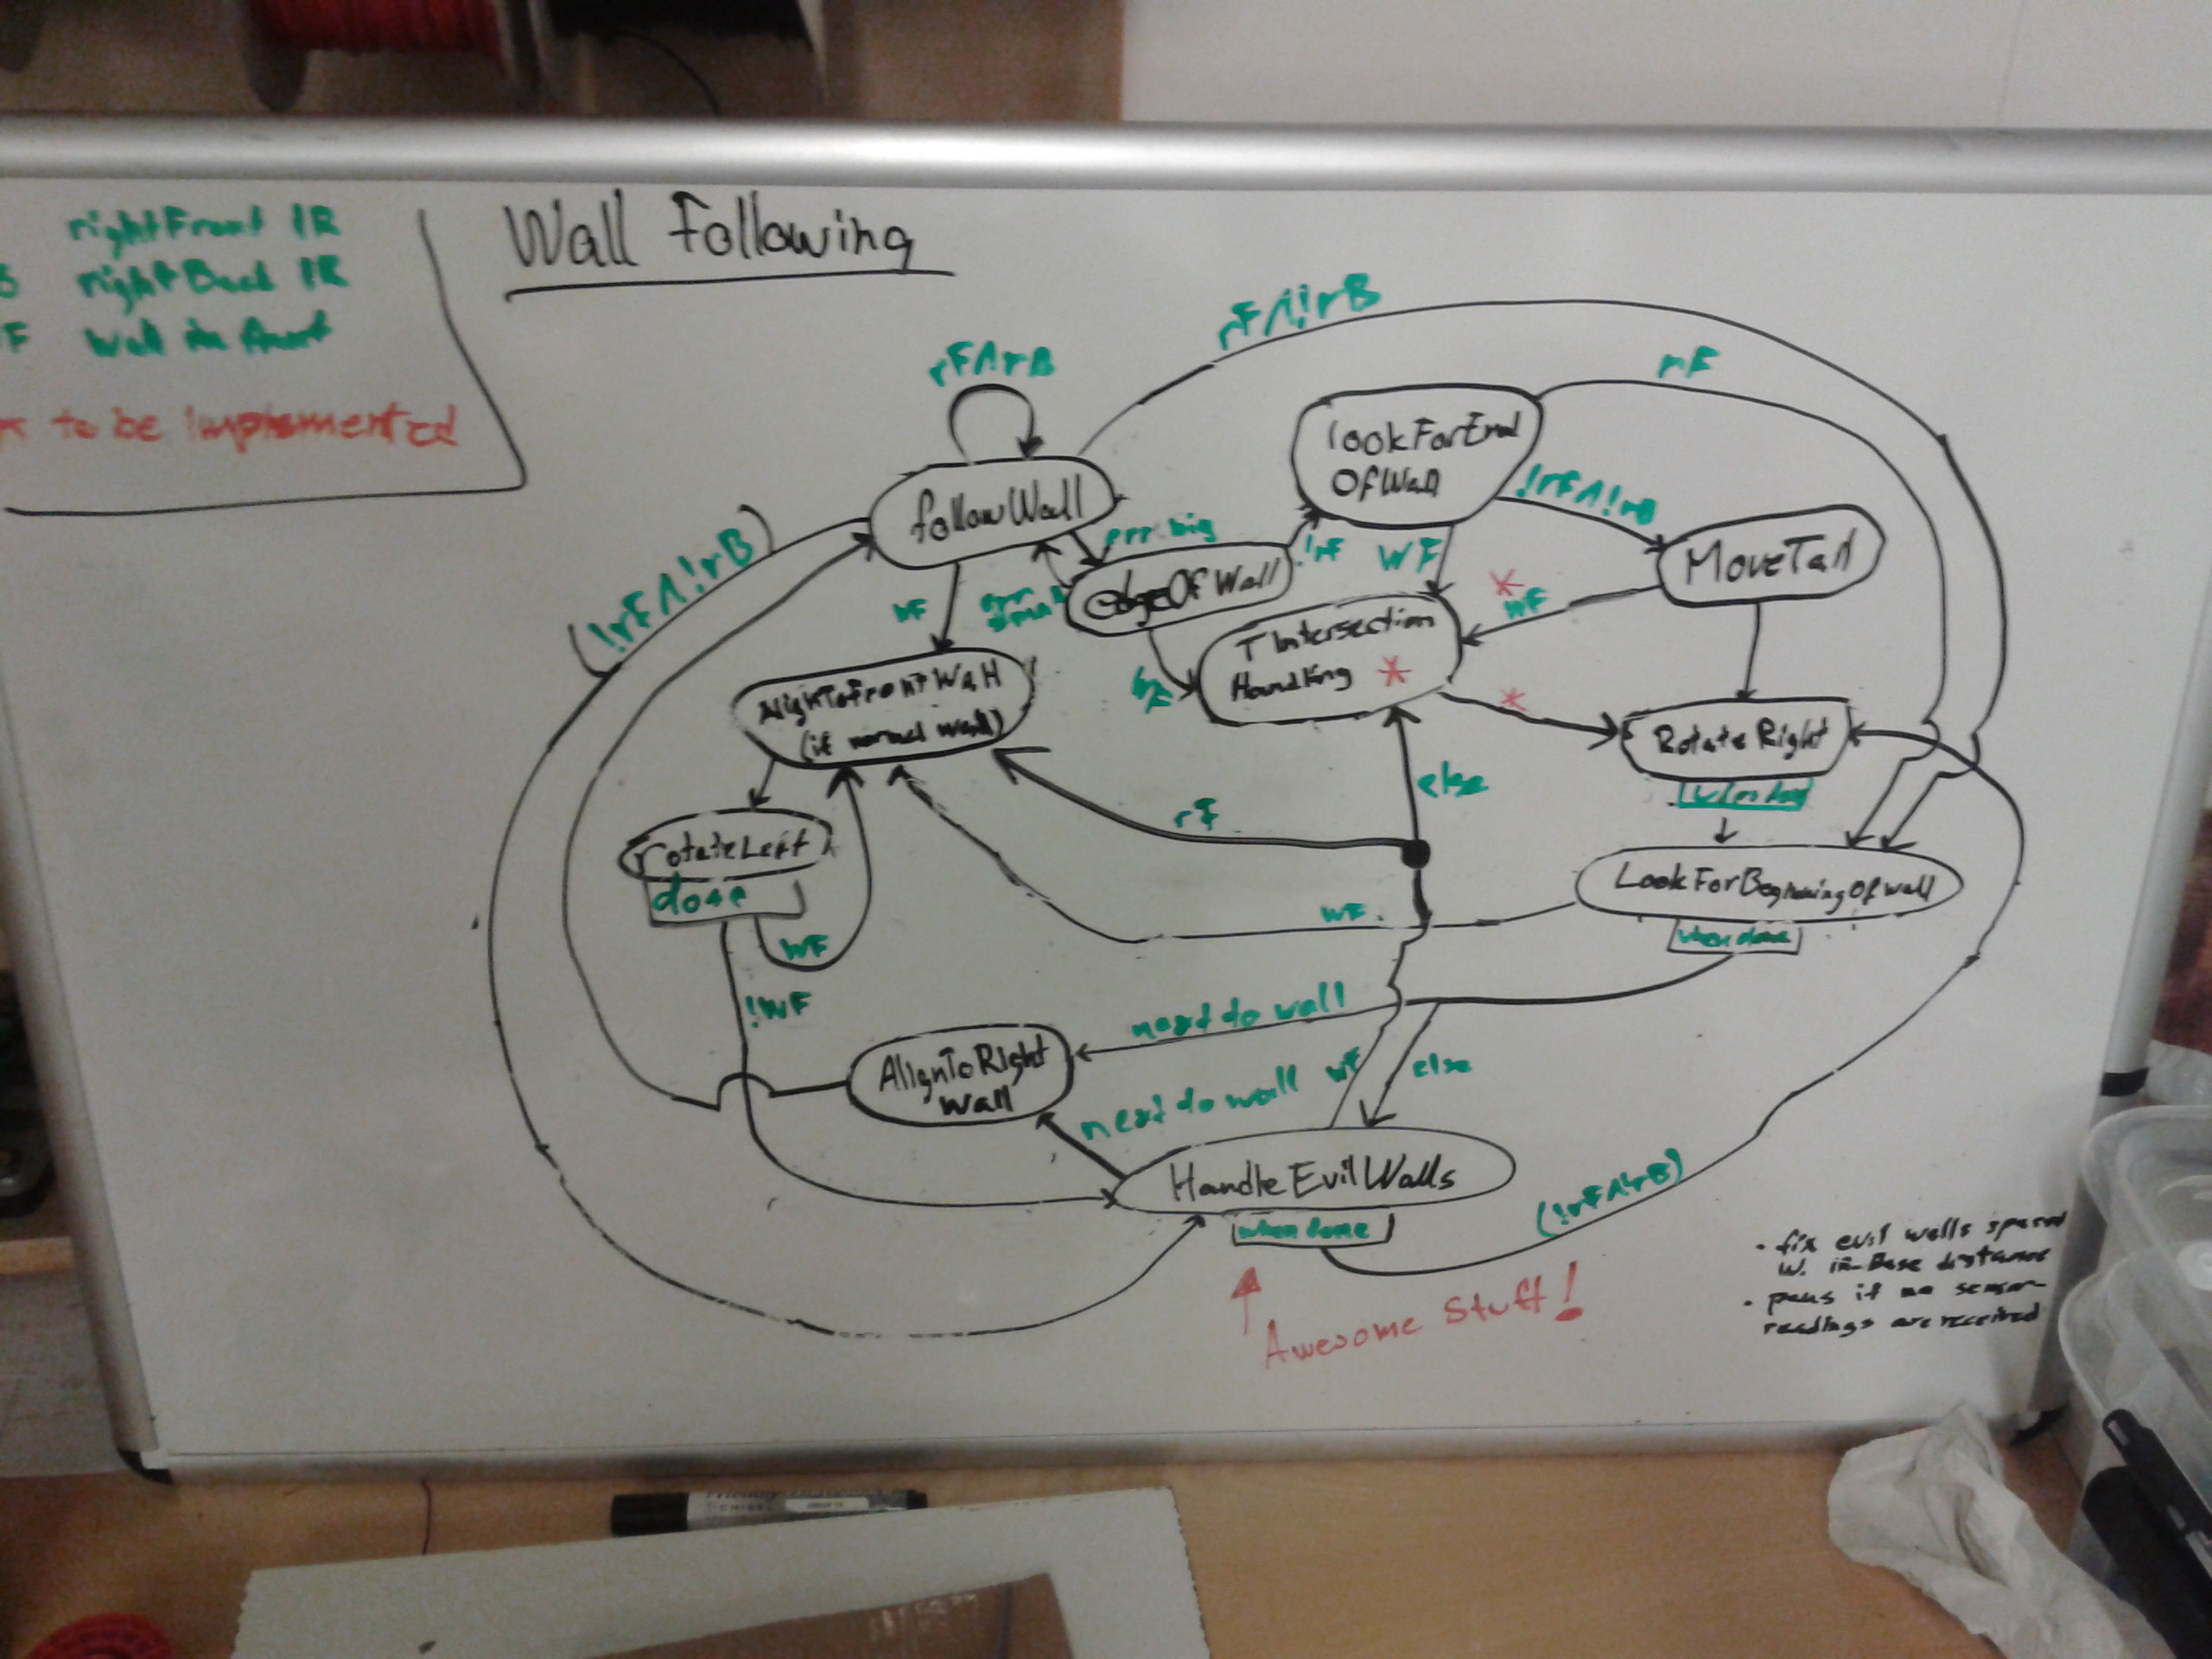
\includegraphics[scale=0.15]{figures/followWallStates.jpg}
   	 \caption{followWallStates, TODO: nice image.}\label{fig:followWallStates}
    \end{centering}
\end{figure}

The states are briefly explained in table \ref{table:followWallStates}. 
\begin{table}
\label{table:followWallStates}
\center
  \begin{tabular}{l|p{10cm}}
    % \hline
    \textbf{State} & \textbf{Description} \\ \hline
    Follow Wall & A state that follows the right wall as long as there is a wall on the robot’s right side. \\ \hline
    Rotate right & Rotates 90 degrees right. \\ \hline
    Rotate left & Rotates 90 degrees left. \\ \hline
    Align to wall & Aligns the robot to the right wall. \\ \hline
    Align to front wall & Moves the robot to a certain distance and aligns it to the front wall. \\ \hline
    Handle evil walls & Drives forward for a certain distance. Every time the front IR on the right side sees a wall, this distance is increased. \\ \hline
    Move tail & If e.g. the right wall ends, this state moves the robot forward so that it has some clearance to to go around corners. \\ \hline
    Edge of wall & This state prevents the robot form making quick heading corrections when a wall ends and the IR suddenly changes value. \\ \hline
    Look for beginning of wall & Moves straight until both the front and the back IR see the same wall.  \\ \hline
    Look for end of wall & If the robot is following a wall and the right front IR sensor doesn’t see the wall any more, this state is used to drive the robot straight forward until the right back IR doesn’t see the wall either. \\ \hline
    T intersection handling & If the robot detects a wall in front, this state first aligns the robot to the front wall and then switches to Rotate right to check if it’s possible to go right. \\ 
    \hline
  \end{tabular}
\end{table}

The following states handles most situations that could appear in the environment.

\subsection{Move to coordinate}

Sometimes it is necessary to move away from the wall in order to explore the whole environment. Move coordinate is used to do this, it’s based on the same basic functions as the wall following function is based on, namely the linear movement and the angular movement. As the name tells it moves to a specified coordinate by first rotating and then move straight to that point.

\subsection{Movement control}

Movement control uses all the functionality previously described here in section \ref{sect:motionControl} to be able to make any movement that is required, follow wall and move to coordinate, to explore the whole environment.

\section{Mapping and Localization}
The localization and the mapping of the maze are done by a node called Mapper.
It runs at a frequency of $30Hz$ and maps all walls detected by the IR-sensors based on the current pose estimation. The pose is a three dimensional vector $(x,y,\theta)$ describing the robot's position and orientation in a global coordinate system. The pose estimation is mainly based on odometry data. Since this data drifts the Mapper tries to reduce the error by taking the IR data into account.


\subsection{Map}
The maze is built out of linear wall segments and any angle between two non parallel walls is $\frac{\pi}{2}$.
Thus it is possible to separate all walls into two classes: horizontal and vertical walls. Horizontal walls are defined to have an angle of $0$ and vertical walls $\frac{\pi}{2}$. 
The map data structure is based on this constraint and consists out of a list of vertical and horizontal wall segments.

Each wall segment consists out of two points: one start point and one end point. In case of a vertical wall these points have the same $x$-coordinate and in case of a horizontal wall the same $y$-coordinate. For convenience it is defined that the start point has the lower $x$($y$)-coordinate and the end point the higher one.

\subsection{Mapping}
The mapping is done while wall following. Since the angles of the walls are strictly defined to be either $0$ or $\frac{\pi}{2}$ the mapping can only be started once the robot is aligned parallel to a wall. As described in section \ref{wallFollower} the wall follower has $11$ different states. Every time it changes its state it publishes a message that is received by the Mapper. The first time the wall follower leaves the state \textit{AlignToWall} the Mapper starts mapping. The pose the robot has when this event occurs is defined to be $(0,0,0)$. From there on the pose is first updated based on odometry and then corrected by the mapper as described in section \ref{Localization}.
Amee has four short range IR sensors, two on each side. Each sensor is handled separately. Based on the current pose the measured distance is used to calculate the position of where the IR beam is reflected. The approach described in section \ref{dataAssoc} for data association is then used to associate this measurement with a previously mapped wall. If no wall fits a new wall segment is added to the map at this position. The orientation of this new wall segment depends on the current orientation of the robot.

The map stores each type of wall segments in its own list. The list of horizontal walls is ordered by increasing $y$-coordinates and the list of vertical walls by increasing $x$-coordinates. This allows walls that have almost the same $x$(or $y$)-coordinate and overlap or are close to each other to be merged. This compensates drift in the pose estimation and is necessary to merge two wall segments of which one is mapped by the front sensor and the other by the back sensor on one side. 

\subsection{data association}
\label{dataAssoc}
The data association is done by ray tracing. Each wall is represented by a line from its start point to its end point. The IR-measurement defines together with the position of the sensor another line, the IR beam. To associate a measurement to a wall it is checked for each wall if the beam and the wall intersect. In case of an incorrect pose estimation it might be that the beam intersects with multiple walls. In that case the measurement is associated to the closest wall to the sensor's position. To allow the wall to grow and to deal with some error in the IR distance both the beam and the wall are artificially enlarged for a couple of $cm$ for this calculation. TODO: image?    

\subsection{Localization}
\label{Localization}
If the data association for both the front and the back sensor on one side is succesful it is possible to correct two components of the pose. The angle relative to the wall can be calculated as $\theta_{rel} = \arctan(\frac{d_{f} - d_{b}}{b})$, where $b$ is the distance between the front and the back sensor, $d_f$ and $d_b$ the measured distances at the front and at the back. Depending on the type and the side of the wall the robot is on, the absolute angle of the wall is either $0$, $\frac{\pi}{2}$,$\pi$ or $\frac{3 \pi}{2}$. With these it is possible to calculate the absolute angle of the robot $\theta$.

If the robot is next to a horizontal wall it is further possible to adapt the robot's $y$-position. In case of a vertical wall it's the $x$-position.
The respective coordinate can be reset based on the measured distance to the wall and the coordinates of this wall. Due to ray tracing it is possible to correct the pose in both cases if it's estimated too close and too far from the wall.

\subsection{Graph}

For path planning a roadmap defined as directed visibility graph on the map is used. The graph's nodes are placed where one of the following events occurred while mapping: the wall follower aligned to a wall, rotated left or rotated right or a tag was detected. 
The camera node described in section \ref{ComputerVision} notifies the mapper node about any tag detection. To prevent multiple tag entries into the map at the same position due to multiple detections of the same tag, a tag node is only added if it is at least $0.08m$ away from the last detection. 
The first node added to the graph denotes the entry/exit of the maze.
Each node has an id which uniquely identifies it. The ids are increased every time a new node is added and thus represent the order in which the nodes are added.

\subsection{Edges}

By default the nodes of the graph are connected in the order they were added. Thus they represent exactly the path the robot drove while mapping. Once the mapping is done additional edges are added. Two nodes $n_1,n_2$ are connected by an edge $(n_1,n_2)$ if the following requirements are fulfilled:
\begin{itemize}
 \item their distance is less than $0.5m$
 \item $n_1 < n_2$
 \item there is a collision free linear path from $n_1$ to $n_2$.
\end{itemize}

The reasons for the first two constraints are explained in section \ref{pathplanning}. The collision checks are executed on the map. For this the line connecting $n_1$ and $n_2$ is sampled. On each sample point the shortest distance to any wall from this point is calculated. This distance is the radius of a collision free circle around the sample point. If it is bigger than the robot's radius plus a small margin, this point can be part of a collision free path, if not it can not and there is no path. This is done for a limited number of sample points until either the complete path is guaranteed to be collision free or a collision was detected.
TODO: provide image

\subsection{Exploring grid}
The map does only store where walls have been measured, but not where the robot 
has been and where not. It is not guaranteed that the robot will pass all walls inside
of a maze just by wall following. Instead it might occur that there are some areas inside of the
maze that are only reachable by moving freely into unexplored space without following any wall.
To be able to detect such regions an additional data structure called exploration grid used.
The exploration grid is a binary grid map that stores for cells of a size of
$10cm*10cm$ if they have been explored by the robot or not.
While mapping a cell is set to be explored if one of the following conditions is met:

\begin{itemize}
\item it intersects with the robot
\item it lies between the robot and a cell in which a wall is measured
\item it contains a measured wall on the right side of the robot
\end{itemize}



\subsection{Evaluation}

The implemented mapper node performed in both mapping and localizing very well. The maps of the test mazes turned out to have only few errors, which do not affect the robot’s overall performance. The localization works very well as long as the robot does not move far away from any wall for a longer time period. 
Even if the position drifted, the localization can still recover from it by doing wall following for a time.
The implemented map data structure allows to map mazes with an arbitrary size without requiring any a priori knowledge about it. The representation as set of linear wall segments turned out to be very advantageous as it requires only few memory and allows efficient calculations for the pose correction and collision checking. 
The exploring grid, however, as simple implementation of a grid map adds a lot of disadvantages. It has a predefined maximum number of cells and thus constraints the possible size of mazes the robot can deal with. Although the resolution of the grid is quite low, it needs more memory than the map of the walls.

If the robot is next to a wall, it is only possible to correct two out of three components of the pose. While $\theta$ can always be corrected $x$ can only be corrected if the robot is next to a vertical wall and $y$ can only be corrected if it is next to a horizontal wall. Thus if the robot drives parallel to the same wall for a long time, the not corrected component of the pose drifts as it is purely based on odometry.

As one can see in image \ref{TODO: image of map} the mapper does not map corners. This is due to the way the data association is done. When the robot is rotating in a corner for the first time only one of both walls exist in the map. After the robot rotated approximately $45^{\circ}$ the IR measurements that belong to the new wall are still associated to the existing wall. This would result in As the mapper tries to correct the robot’s orientation based on the 
no corners mapped 

\subsection{Possible improvements}

\section{Strategies}
In this section high level strategies are presented. These high level strategies include a strategy for path planning and execution, a strategy of
how to explore a maze and one of how to collect tags that have been previously mapped. The different strategies and their functionality are summarized in table \ref{table:strategies}.

\begin{table}[h]
\label{table:strategies}
\center
  \begin{tabular}{l|p{10cm}}
    % \hline
    \textbf{Strategy} & \textbf{Description} \\ \hline
    StrategyGoto & Plans a path from the current position to a given node and executes it.  \\ \hline
    StrategyExplore & Explores a maze by doing wall following and moving to unexplored regions once the robot fully explored one wall. \\ \hline
    StrategyCollect & Collects tags that are stored in the graph. \\
    \hline
  \end{tabular}
\end{table}

Although these strategies are required to fully solve the task, they have not been successfully implemented. The in subsection \ref{subsec:goto} presented StrategyGoto is the only one that was implemented. In subsection \ref{subsec:conceptsStrategies} the concepts for the strategies for exploring and collecting tags are shortly presented.

The idea was that all higher level strategies are executed by a node called StrategyControl. Each strategy is one state of StrategyControl. 
The states for exploration and tag collection require the functionality provided by StrategyGoto. Therefore each state is encapsulated in an object which allows to reuse the functionality of StrategyGoto inside of StrategyExploration and StrategyCollection. It is basically the same design pattern as used for MovementControl.

\subsection{StrategyGoto}
StrategyGoto plans a path on the graph provided by the Mapper node from the current position to a given node that is identified by its id.
\subsubsection{Path planning}
\label{pathplanning}
The path planning is completely done on the graph provided by the Mapper node. Each edge in the graph describes a linear collision free path between the nodes it is connecting. Although each edge $(n_1,n_2)$ could be bidirectional they are set to be unidirectional so that $n_1 < n_2$. The reason for that lies within a weakness of the path execution and is explained in more detail in \ref{subsubsec:pathExec}. 

To find a shortest path on the graph a modified Dijkstra algorithm is used. The modification lies within the calculation of the distance between two nodes $n_1, n_2$ that are connected by an edge $n_1, n_2$:

\begin{equation}
 	d_{n_1,n_2} = 
		\begin{cases}
			\sqrt{(x_{n_1} - x_{n_2})^2 + (y_{n_1} - y_{n_2})^2} & \text{if } n_2 - n_1 = 1 \\
			1.5 * \sqrt{(x_{n_1} - x_{n_2})^2 + (y_{n_1} - y_{n_2})^2} & \text{else }
		\end{cases}
\end{equation}  

This modification results in a non optimal path. However, it prevents the path to contain a lot of shortcuts. A shortcut is an edge that requires the robot to move freely without following a wall. While such edges are the only way the found path can differ from simple wall following, they also bear a higher risk of getting lost or colliding with the environment.

\subsubsection{Path execution}
\label{subsubsec:pathExec}
The path execution is done by using two basic movements: following a wall and moving freely to a certain position. Both functionalities are provided by the MovementControl node. Following a wall has significant advantages against moving freely. The wall follower reacts on all kinds of sensor input to follow a wall without any collisions. Further the localization based on odometry can only be improved by the Mapper node if the robot moves close to a wall. If the robot moves freely far from any wall the pose estimation is purely based on odometry. This can result in severe drift in the pose estimation which makes it hard to navigate further. 

Therefore it is preferable to follow the wall as often as possible and taking as few and as short shortcuts as possible even if this means that the path is by far not the shortest. 
A segment of a path along each edge $(n_1, n_2)$ for that $n_2 - n_1 = 1$ is true can be executed by following a wall. 
Any segment of a path along an edge $(n_1, n_2)$ with $n_2 > n_1 + 1$ is a shortcut. 

Since the wall follower can only follow a wall on the right side of the robot, edges $(n_1, n_2)$ with $n_2 < n_1$ are forbidden and not part of the graph. A shortcut is taken by moving the robot freely from the first node to the second. To reduce the risk of getting lost while taking such a shortcut the maximal length of shortcuts is set to $0.50m$.   

The result of the path planning is a sequence of nodes the robot has to move to to get to its final destination.
Depending whether the next node can be reached by following a wall or taking a shortcut the respective command is sent to MovementControl.
If the next node can only be reached by moving there freely, the direction and the distance from the current pose to the node's pose is calculated. The robot then rotates first and then moves straight for the calculated distance. 

If the next node can be reached by following a wall, the wall follower is executed until the Mapper signals that the desired node has been reached.

If the next node is a tag, the current pose is compared with the nodes' pose.

Once the next node is reached, a new command is issued to get to the next node in the sequence. This is repeated until the final node has been reached.

The path execution worked in some cases, but also failed in many other cases. Due to navigational errors by moving freely it often happened that the wall following was started at a different position then where the node actually was. In case of a tight maze this could result in a different sequence of wall following events. This could result in never reaching a node just because the wall follower didn't have the same state transition at this position as stored in the node. Setting a node to be reached because the robot has reached its pose as it is done for tag nodes might have been a better solution. It was expected that the pose estimate is a less reliable localization than the wall following events which turned out to be wrong.    


\subsection{Concepts for Phases}
\label{subsec:conceptsStrategies}
\subsubsection{Exploration}
In exploration strategy our robot follows a wall until it has come to an ealier position with the same angular direction. If so, that means that the robot is moving in circles. It then stops and looks for other positions in the graph where it has not yet been, and looks for a collision free path from any node in the graph to that position. That position is chosen by first finding all non visited blocks (called ''blobs'') and then choose the next biggest one (because probably the biggest one is outside the maze).
In our current implementation this functionality is not fully integrated.

\subsubsection{Collection}

\section{ComputerVision}
\label{computerVision}
The overall goal of the computer vision part of the robot is to constantly analyze its surroundings, try to find the locations of tags and classify those (i.e determine what is is). The system should then send the results to the rest of the robot system which in turn stores location and type of object on a map.

The surroundings of the robot in the sense of computer vision is defined to be the field of view of the camera mounted in a position overviewing the right side of the robot. A tag is a picture of some object (from a predefined set of objects) located within a red rectangular border. In addition to determine class of object we also have to decide the color of the object.

To get raw camera feed we used a library that directly talked to the camera by using the V4L2 driver for image capturing this since the driver provides the best performance (i.e. the minimum delay) and the ability to sidestep internal camera buffers to get higher throughput. Still the delay between a retrieved image and real-time observed scene remained around 0.5s. Due to limitations in computational power in the hardware used it was only possible to receive and decode about 2 to 3 frames per second from the attached camera.

To accomplish the above goals we investigated three different procedures: classification using SURF (Speeded Up Robust Features) and template matching, for color detection: simple summation of pixels. While a SURF based approach is interesting due to generally good results it did not work in our case (see section 'SURF') and the final method of choice was to use template based matching.

\subsection{Finding Tags}
As already mention, computer vision is very calculation intensive. We can't expect to analyze every frame received from the camera completely, instead we want to grab the a frame and quickly determine if there maybe could be a tag in the frame and if so continue analyze the frame further with the hope of actually finding a tag. The procedure was as follows, when in normal mode (i.e. driving around looking for tags) capture a low resolution frame as often as possible. In the frame received make a single pass and calculate the number of red pixels, if this number is above some threshold conclude that there is a tag in current frame. If a tag has been found change state and continue analyzing the frame.

There are some things here that need some clarification. Given the predefined structure of the maze with white walls and a camera mounted on the robot pointing directly on on the wall we can be absolutely certain the a captured frame will only contain either: only the white wall or a (part) of a tag with the white wall as background. Since our goal is to calculate the number of red pixels in each frame and there can be no other source of red except a possible tag in the frame we can conclude that the only important statistic needed is the ratio between (possible) red pixels and the white pixels from the background. This means that tag finding is independent of resolution of captured frame! Using this fact we can now capture a low resolution frame (which requires less calculations) and still be certain of the result with the gain of huge speed improvement. We used a resolution 160x120 pixels to get better statistical significance but could probably have used even lower resolution but this was not tested.

We now need to determine when is a pixel red? One of the hardest problems in digital image segmentation is lightning. Depending on the lightning condition a pixel can look completely different, for example in a bright room a red pixel could have a warm red tone but in a dark room it looks almost blue. By switching to a different color model, such as the HSV (Hue, Separation, Value) we can separate color from light intensity. 

When using the hue component of a color, it is always important to take its saturation into account (which is the second entry of the vector). Indeed, when the saturation of a color is low, the hue information becomes unstable and unreliable. This is due to the fact that for low-saturated color, the B, G, and R components are almost equal. This makes it difficult
to determine the exact color represented. 

As shown the HSV model is not perfect either and due to unavoidable noise and errors in image capturing a range of valid red colors had to be established through empirical investigation. The threshold value for how many red pixels that needs to be present in frame to constitute a tag was also established empirically. Having found a frame that with high probability might contain a tag we can now switch state and try to classify it.

\subsection{Classification using SURF}
SURF (Speeded Up Robust Features) is a robust local feature detector (or descriptors) used to find blobs in images (a blob here simply means a chunk of pixels for which you can form some form of group).  A descriptor is a scalar that describes a shape on some way, this could be the sum of a histogram, area of blob or even more advanced functions. A shape (or blob) may not be reconstructable from the descriptors, but the descriptors for different shapes should be different enough, so that shapes can be discriminated.

Pros of using SURF is that it is both scale and rotation invariant due to clever calculations of image descriptors, how these descriptors is calculated is pretty advanced and will not be covered. SURF descriptors are fine for comparing richly textured images since it is then easy to calculate many descriptors.

The tags we where supposed to classify did not contain this rich structure and it proved to be difficult to get the algorithm to generate more than around five or six good and unique descriptors. When we tried to match a captures tag image against the set of all valid tags using descriptors the degree of certainty was extremely low. 

It is highly likely that it is possible to improve our naive usage of SURF to get better results but due to time limitations we abandon the idea and instead went for the much more battle hardened approach of template matching as explain earlier.

\subsection{Classification Using Template Matching}
When classifying tags we try to be as efficient as possible. Our ultimate goal is to classify tags using a template based approach but before that is possible there are numerous steps to go through. We carry out the procedure by dividing up the the classification process into a pipeline which can be broken at almost anytime upon reaching a state where we conclude a false positive (i.e no tag in frame or it is impossible to classify correctly) we then break and return to looking for new tags to avoid unnecessary and costly operations. The pipeline is constructed as follows:

Find red pixels in image (already covered)
Find (possible) tag region of interest (Canny edge detection, contour optimization)
Prepare region of interest (remove border, resize)
Classify using templates (blur, threshold, match against templates)
Determine tag color (count pixels in region)

First we need to find the location of the tag in the image. This is done by first using the 'Canny' edge detection algorithm which is considered to be the state-of-the-art algorithm for edge detection. We then locate all the contours in this resulting binary image. By using previously established knowledge about the size of tags and approximative distance between camera and the wall, we calculate what an approximative area of a tag in this region would be, compare with found contours and pick the one which match this criteria. 

To achieve higher certainty in finding contours a set of morphological operators was applied to the binary image to make sure that shapes really consists of a set of connected components. A single pass of a dilation mask was enough.

If a suitable region was found cut out this region of interest (hereafter referred to as ROI) and throw away the rest. Experiments show that this ROI tends to be around 60x60 pixels. 

Before explaining the next step (prepare ROI) we have to understand the reason behind it. The basic idea behind template matching is to take an image and let a another smaller image (the template) 'slide' over. The region of the original image where the template has the best match (with some degree of error) is considered the winning region. If we where to match agains several templates (which we will) we simply repeat the same procedure with each tag and the one with smallest error is considered to be the best match.

Now, given a set of predefined tags, if we where to make sure that all templates, and the possible tag we would like to match against, would have the same size it means that we could skip the step of 'sliding' one image over the other and limit ourselves to doing one matching per template to calculate the error degree for each template. The template with the smallest error is clearly the best match and the image can now be classified according to this match. Continuing this idea of same structure, when initializing the templates we convert them all to a resolution of 50x50, threshold them into binary images and make sure the border around each template is completely removed to make sure we have as simple structure as possible.

Returning to the (possible) tag in a ROI. The prepare step consist of executing this previously explained procedure. The only difference is we have to take factors such as rotation, skew, if the ROI contains borders or not, into consideration. The result is a ROI with same structure as the set of templates, namely: binary image of size 50x50 pixels.

The classification is now easy, we simply loop through and match agains each template, best match is the winner. If the error vector is to big we can't make any conclusions with enough level of certainty so we classify the tag as 'UNKNOWN'. A question the reader now should be asking themselves is: ''Would higher resolution of tags/templates give higher degree of certainty in the results?''. We tested with resolutions up to around 300x300 for the tag ROI and templates with an source image resolution of 640x480 and the answer is no. The end result was that we where able to correctly classify the same amount of tags with high resp. low input resolutions. The question is still open for even higher resolution, in which we believe the results would be better, but the tradeoff with the extreme increase in computational cost it was not considered to be worth it.

\subsection{Color Detection}
To determine the color of the now classified object. Since we know that the color of a tag would be one of four previously defined colors simply sum up the number of pixels belonging to different color categories and the one with highest sum is the resulting color class. To reduce the amount of noise and to make sure we did not take border pixels into account we sampled a small region of the center (30\% going outwards) of the tag ROI this was possible since every source tag contained colors pixels in the middle.

We found the intervals for the different color regions by empirically studying histograms of captured frames for various tag colors and it worked surprisingly well for the distinct colors of green, blue and magenta. Detecting black colors proved to be much more difficult (since black is the absence of all colors). Since every capture image contains noise and a black color vector doesn't have any magnitude we instead used a little trick: if the capture ROI consists of an even spread (the amount of pixels will be low) of colors for green, blue, magenta we conclude that the object must be black. This also worked very well and from experiments we detect the correct color in roughly 9 of 10 cases.

\section{Future work}
Movement control: The linear movement can be improved by implementing the same acceleration limitation as the angular movement function uses to make the movement even smoother.
	If the complexity of the environment increases one should consider another method of exploring the environment than wall following in the sense it’s implemented now. A more complex environment would need many more states to be able to handle all possible situations and a more complex state machine will be very hard to debug. 

\section{Evaluation}
The robot turned out not to provide all the functionalities to fully fulfill the tasks.

The overall movement control of the robot performed well and the wall following can deal with a lot of different wall constellations while moving fast and close to the walls.
The localization and mapping as well performed very well in many tests. Though there are still some possible improvements which were presented in the respective section.

The computer vision performed apart from difficulties due to differnt lightning conditions also very well. It was possible to correctly classify a number of tags without even stopping the robot.

Due to the lack of time we did not manage to fully integrate all the functionalities into different high level strategies for exploring the maze and collecting tags. The path execution is still not stable and reliable why it wasn't even used during the competition. 

Thanks to the fast wall follower and to the fast computer vision we still managed to get through the maze in the competition in time and detect and classify at least some tags. 

\section{Conclusion}
Well, Amee isn't as good as the Terminator yet, but Arnie wasn't build in one month either...

\clearpage
\begin{thebibliography}{9}

%\bibitem{lamport94}
%  Leslie Lamport,
%  \emph{\LaTeX: A Document Preparation System}.
%  Addison Wesley, Massachusetts,
%  2nd Edition,
%  1994.
  
\bibitem{ros_home}
  ROS wiki
  \url{http://www.ros.org/wiki/}
  
\bibitem{course_wiki}
  Course wiki
  \url{https://anywiki.csc.kth.se/DD2425/doku.php}
  
\bibitem{ros_home}
  Sketchup
  \url{http://www.sketchup.com/}
  
\bibitem{open_cv}
  OpenCV
  \url{http://opencv.org/}
  
\bibitem{amee_video_evilwall}
  Amee video evil wall detection
  \url{http://www.youtube.com/watch?v=vI2VA1gsv2g}
  
\bibitem{amee_video_contest}
  Amee video on contest
  \url{http://www.youtube.com/watch?v=_6EvMS079ZM}
  
\bibitem{source_code}
  Source code
  \url{https://github.com/wejeus/robot12/}

\end{thebibliography}

\end{document}
